%%%%%%%%%%%%%%%%%%%%%%%%%%%%%%%%%%%%%%%%%%%%%%%%%%%%%%%%%%%%%%%%%%%%%%%%%%%%%%%%
% LaTexThesisTemplate, Author: Johannes Muenichsdorfer and Technical University of Munich (TUM)
%%%%%%%%%%%%%%%%%%%%%%%%%%%%%%%%%%%%%%%%%%%%%%%%%%%%%%%%%%%%%%%%%%%%%%%%%%%%%%%%

%%%%%%%%%%%%%%%%%%%%%%%%%%%%%%%%%%%%%%%%%%%%%%%%%%%%%%%%%%%%%%%%%%%%%%%%%%%%%%%%
\documentclass[%
    fontsize=11pt, % Schriftgröße
    twoside=off, % kein einseitiges Layout
    bibliography=totocnumbered % bibliography has chapter number and shows in the toc
]{scrbook} % Dokumentenklasse: KOMA-Script Book
\usepackage{scrlayer-scrpage} % Anpassbare Kopf- und Fußzeilen

\usepackage[utf8]{inputenc} % Textkodierung: UTF-8
\usepackage[T1]{fontenc} % Zeichensatzkodierung

\usepackage{wrapfig} % Wrapping Images and Text
\usepackage{graphicx} % Grafiken
\usepackage[dvipsnames]{xcolor} % Colors

% Schriftart Helvetica:
\usepackage[scaled]{helvet}
\renewcommand{\familydefault}{\sfdefault}

% Silbentrennung:
\usepackage{hyphenat}
\hyphenation{TUM in-te-res-siert} % Eigene Silbentrennung
%\tolerance 2414
%\hbadness 2414
%\emergencystretch 1.5em
%\hfuzz 0.3pt
%\widowpenalty=10000     % Hurenkinder
%\clubpenalty=10000      % Schusterjungen
%\vfuzz \hfuzz

\usepackage[onehalfspacing]{setspace} % 1,5facher Zeilenabstand
\usepackage{calc} % Berechnungen
\usepackage{enumitem} % Mehr Kontrolle über itemize-, enumerate- und description-Umgebungen
\usepackage{relsize} % Schriftgröße in Abhängigkeit von aktueller anpassen
\usepackage{tabularx} % Flexiblere Tabellen
\usepackage{colortbl} % Tabellen Farbig
\usepackage{caption} % Anpassen von Beschriftungen

% Nummerierung von Abbildungen & Tabellen durchgängig, statt nach Kapiteln:
\usepackage{chngcntr}
\counterwithout{figure}{chapter}
\counterwithout{table}{chapter}

% Abkürzungen, Glossare:
\usepackage[%
    xindy,% xindy zum Indexieren verwenden
    acronym,% Separates Akronym-Verzeichnis
    nopostdot,% Kein Punkt am Ende einer Beschreibung im Glossar
]{glossaries}

% Code render package:
\usepackage{listings}

% Spezielle Befehlsdefinitionen:
\newcommand{\Topic}{}
\newcommand{\savefootnote}[2]{\footnote{\protect\label{#1}#2}} %Save a repeating footnote
\newcommand{\repeatfootnote}[1]{\textsuperscript{\ref{#1}}\normalfont} %Display a repeated footnote

% Links und Fußnoten: 
\usepackage{footnotebackref}
\usepackage{hyperref} % Hyperlinks (needs to be the last package to be imported)

% Debugging:
%\usepackage{showframe} % Layout-Boxen anzeigen
%\usepackage{layout} % Layout-Informationen
%\usepackage{printlen} % Längenwerte ausgeben
 % !!! DO NOT REMOVE !!!
%%%%%%%%%%%%%%%%%%%%%%%%%%%%%%%%%%%%%%%%%%%%%%%%%%%%%%%%%%%%%%%%%%%%%%%%%%%%%%%%

\renewcommand{\Topic}{IDP Report - Mark Robotics - Precision Line Marking Detection} % !!! ADD YOUR TOPIC HERE !!!

%%%%%%%%%%%%%%%%%%%%%%%%%%%%%%%%%%%%%%%%%%%%%%%%%%%%%%%%%%%%%%%%%%%%%%%%%%%%%%%%
%%%%%%%%%%%%%%%%%%%%%%%%%%%%%%%%%%%%%%%%%%%%%%%%%%%%%%%%%%%%%%%%%%%%%%%%%%%%%%%%
% EINSTELLUNGEN
%%%%%%%%%%%%%%%%%%%%%%%%%%%%%%%%%%%%%%%%%%%%%%%%%%%%%%%%%%%%%%%%%%%%%%%%%%%%%%%%

% Sprache:
\usepackage[english]{babel}

\KOMAoptions{parskip=full}

% Seitenränder:

\newcommand{\SeitenrandOben}{25.8mm}
\newcommand{\SeitenrandRechts}{21mm}
\newcommand{\SeitenrandLinks}{40mm}
\newcommand{\SeitenrandUnten}{24.8mm}
\newcommand{\FusszeileHoehe}{11.7mm}

\usepackage[a4paper,
    head=0pt,
    top=\SeitenrandOben,
    bottom=\SeitenrandUnten,
    inner=\SeitenrandLinks,
    outer=\SeitenrandRechts
]{geometry}

% Fußzeilen:

\setlength{\footheight}{\FusszeileHoehe}
\clearscrheadfoot
\ifoot*{\Topic\vfill}
\ofoot*{\pagemark\vfill}
\setkomafont{pageheadfoot}{\fontsize{9pt}{13pt}\normalfont}
\setkomafont{pagefoot}{\bfseries}
\setkomafont{pagenumber}{\normalfont}
\pagestyle{scrheadings}


% Fußnoten:

\KOMAoptions{%
    %footnotes=multiple % mehrere Fußnoten werden durch Zeichen getrennt
}
%\setfootnoterule[.6pt]{5.08cm}
\renewcommand{\footnoterule}{\hrule width 5.08cm height .6pt \vspace*{3.9mm}}
%\setlength{\footnotesep}{5mm}
\deffootnote{2mm}{2mm}{%
    \textsuperscript{\hyperref[\BackrefFootnoteTag]{\thefootnotemark}}\,%
}
\setkomafont{footnoterule}{\fontsize{9pt}{20pt}\selectfont}

% Links und Fußnoten: 
\hypersetup{
	colorlinks,
	linkcolor={red!50!black},
	citecolor={blue!50!black},
	urlcolor={blue!80!black}
}


% Überschriften:

\KOMAoptions{%
    open=any, % keine Festlegung auf linke oder rechte Seite
    numbers=noendperiod, % kein automatischer Punkt nach Gliederungsnummer
    headings=small
}

\makeatletter
\g@addto@macro{\@afterheading}{\vspace{-\parskip}} % \parskip nach Gliederungsbefehlen entfernen
\renewcommand*{\chapterheadstartvskip}{\vspace{\@tempskipa}\vspace{-3pt}} % Korrektur für Abstand über Kapitelüberschriften
\makeatother

\setkomafont{disposition}{\normalfont\sffamily}

\setkomafont{chapter}{\normalfont\fontsize{19pt}{22pt}\selectfont}
\RedeclareSectionCommand[%
  beforeskip=0pt,
  afterskip=29pt
]{chapter}
\renewcommand*{\chapterformat}{\thechapter.\enskip} % Immer Punkt nach Kapitelnummer

\setkomafont{section}{\fontsize{15pt}{17pt}\selectfont}
\RedeclareSectionCommand[%
  beforeskip=0pt,
  afterskip=24.1pt
]{section}
\renewcommand*{\sectionformat}{\makebox[13mm][l]{\thesection.\enskip}} % Feste Breite für Abschnittsnummer und immer Punkt danach

\setkomafont{subsection}{\bfseries\fontsize{12pt}{13pt}\selectfont}
\RedeclareSectionCommand[%
  beforeskip=0pt,
  afterskip=1pt
]{subsection}
\renewcommand*{\subsectionformat}{\makebox[13mm][l]{\thesubsection.\enskip}} % Feste Breite für Unterabschnittsnummer und immer Punkt danach


% Listen:

\setlist{%
    labelsep=0mm,
    itemindent=0pt,
    labelindent=0pt,
    align=left,
    parsep=1.5ex
}
\setlist[itemize]{%
    leftmargin=5mm,
    labelwidth=4.9mm
}
\setlist[itemize,1]{%
    before={\vspace{0.25ex}},
    label={\raisebox{.35ex}{\smaller[2]\textbullet}},
    after={\vspace{-\parsep}\vspace{-.25ex}}
}
\setlist[itemize,2]{%
    label={\raisebox{.35ex}{\rule{.58ex}{.58ex}}}
}
\setlist[enumerate]{%
    leftmargin=10mm,
    labelwidth=9.9mm
}
\setlist[enumerate,2]{%
    label={\alph*.}
}

\setlist[description]{%
%    labelindent=!,
    leftmargin=1em,
    labelwidth=!,
    parsep=0mm,
    partopsep=0mm,
    labelsep=1em,
}


% Verzeichnisse:

\KOMAoptions{%
    %toc=flat, % keine Einrückungen im Inhaltsverzeichnis
    toc=chapterentrydotfill, % Punkte bis zur Seitennummer bei Kapiteln
    listof=entryprefix, % Präfix für Einträge in Abbildungs- und Tabellenverzeichnis
    listof=nochaptergap, % Kein Abstand für Kapiteleinträge in extra Verzeichnissen
}

\makeatletter
\renewcommand{\@dotsep}{.3} % Abstand der Füllpunkte

% "chapteratlist" für Inhaltsverzeichnis auswerten:
\renewcommand*{\addchaptertocentry}[2]{%
  \iftocfeature{toc}{chapteratlist}{}{%
    \addtocontents{toc}{\protect\vspace{-10pt}}% extra Abstand vor Kapitelüberschriften in Inhaltsverzeichnis entfernen
  }%
  % Originaldefinition aus scrbook.cls:
  \addtocentrydefault{chapter}{#1}{#2}%
  \if@chaptertolists
    \doforeachtocfile{%
      \iftocfeature{\@currext}{chapteratlist}{%
        \addxcontentsline{\@currext}{chapteratlist}[{#1}]{#2}%
      }{}%
    }%
    \@ifundefined{float@addtolists}{}{\scr@float@addtolists@warning}%
  \fi%
}
\makeatother

\AfterTOCHead[toc]{\protect\vspace{.8ex}} % Abstand zwischen Überschrift und Inhaltsverzeichnis
\setuptoc{toc}{noparskipfake} % Angleichung der Abstände nach Inhaltsverzeichnisüberschrift an andere Überschriften
\unsettoc{toc}{chapteratlist} % kein Abstand vor Kapiteleinträgen im Inhaltsverzeichnis, funktioniert nur durch obige Redefinition von \addchaptertocentry

% -- Abbildungs- und Tabellenverzeichnis:

\AfterTOCHead[lof]{\protect\vspace{-.1ex}\doublespacing} % Abstand zwischen Überschrift und Abbildungsverzeichnis, doppelter Zeilenabstand
\setuptoc{lof}{noparskipfake} % Angleichung der Abstände nach Abbildungsverzeichnisüberschrift an andere Überschriften

\AfterTOCHead[lot]{\protect\vspace{-.1ex}\doublespacing} % Abstand zwischen Überschrift und Tabellenverzeichnis, doppelter Zeilenabstand
\setuptoc{lot}{noparskipfake} % Angleichung der Abstände nach Tabellenverzeichnisüberschrift an andere Überschriften

% Beschriftungen:
\DeclareCaptionFormat{WissenschaftlicheArbeiten}{\fontsize{8pt}{10pt}\selectfont#1 #2#3\par}
\DeclareCaptionLabelFormat{WissenschaftlicheArbeiten}{\bfseries\selectfont#1 #2}

% -- Tabellen:
\captionsetup[table]{%
    format=WissenschaftlicheArbeiten,
    labelformat=WissenschaftlicheArbeiten,
    labelsep=none,
    singlelinecheck=off,
    justification=raggedright,
    skip=3pt,
    tablewithin=none
}

% -- Abbildungen:
\captionsetup[figure]{%
    format=WissenschaftlicheArbeiten,
    labelformat=WissenschaftlicheArbeiten,
    labelsep=none,
    singlelinecheck=off,
    justification=raggedright,
    skip=6.6mm,
    figurewithin=none
}


% Tabellen:
\renewcommand{\arraystretch}{1.8} % Skalierung der Tabellen
\newcolumntype{M}{X<{\vspace{4pt}}} % Spaltentyp mit Abstand rechts


% Glossare & Abkürzungsverzeichnis:

\makeglossaries
\newacronym{acs}{acs. service}{accessibility service}
\newacronym{ace}{acs. event}{accessibility event}
\newacronym{aces}{acs. events}{accessibility events}
\newacronym{aapp}{Android app}{Android application}
\newacronym{aapps}{Android apps}{Android applications}
\newacronym{app}{app}{application}
\newacronym{apps}{apps}{applications}
\newacronym{imes}{IME service}{InputMethod service}
\newacronym{ime}{IME}{InputMethod}
\newacronym{ui}{UI}{User Interface}
\newacronym{www}{WWW}{World Wide Web}
\setacronymstyle{short-long}

\makeatletter
\newlength{\@glsdotsep}
\setlength{\@glsdotsep}{\@dotsep em}
\newcommand*{\glsdotfill}{\leavevmode \cleaders \hb@xt@ \@glsdotsep{\hss .\hss }\hfill \kern \z@}
\makeatother

\newglossarystyle{WissenschaftlicheArbeiten}{%
  \setglossarystyle{index}%

  \renewcommand*{\glossaryheader}{\vspace{.75em}}%
  \renewcommand*{\glstreenamefmt}[1]{##1}%
  \renewcommand*{\glossentry}[2]{%
     \item\glsentryitem{##1}\glstreenamefmt{\glstarget{##1}{\glossentryname{##1}}}%
     \ifglshassymbol{##1}{\space(\glossentrysymbol{##1})}{}%
     \space-\space\glossentrydesc{##1}\glsdotfill\glspostdescription\space ##2%
  }%
  \renewcommand*{\glsgroupheading}[1]{%
    \item\glstreenamefmt{\textbf{\fontsize{14}{17}\selectfont\enskip\glsgetgrouptitle{##1}}}\vspace{.3em}}%
}

\setglossarystyle{WissenschaftlicheArbeiten}


%Bibliography:

\bibliographystyle{CustomIEEEtran}


%Codestyle and Settings:
\definecolor{codegreen}{rgb}{0,0.6,0}
\definecolor{codegray}{rgb}{0.5,0.5,0.5}
\definecolor{codepurple}{rgb}{0.58,0,0.82}
\definecolor{backcolour}{rgb}{0.95,0.95,0.92}

\lstdefinestyle{mystyle}{
	backgroundcolor=\color{backcolour},   
	commentstyle=\color{codegreen},
	keywordstyle=\color{magenta},
	numberstyle=\tiny\color{codegray},
	stringstyle=\color{codepurple},
	basicstyle=\footnotesize,
	breakatwhitespace=false,         
	breaklines=true,                 
	captionpos=b,                    
	keepspaces=true,                 
	numbers=left,                    
	numbersep=5pt,                  
	showspaces=false,                
	showstringspaces=false,
	showtabs=false,                  
	tabsize=2
}

% Kotlin definition:
\lstdefinelanguage{Kotlin}{
	comment=[l]{//},
	commentstyle={\color{gray}\ttfamily},
	emph={delegate, filter, first, firstOrNull, forEach, lazy, map, mapNotNull, println, return@},
	emphstyle={\color{OrangeRed}},
	identifierstyle=\color{black},
	keywords={abstract, actual, as, as?, break, by, class, companion, continue, data, do, dynamic, else, enum, expect, false, final, for, fun, get, if, import, in, interface, internal, is, null, object, override, package, private, public, return, set, super, suspend, this, throw, true, try, typealias, val, var, vararg, when, where, while},
	keywordstyle={\color{NavyBlue}\bfseries},
	morecomment=[s]{/*}{*/},
	morestring=[b]",
	morestring=[s]{"""*}{*"""},
	ndkeywords={@Deprecated, @JvmField, @JvmName, @JvmOverloads, @JvmStatic, @JvmSynthetic, Array, Byte, Double, Float, Int, Integer, Iterable, Long, Runnable, Short, String},
	ndkeywordstyle={\color{BurntOrange}\bfseries},
	sensitive=true,
	stringstyle={\color{ForestGreen}\ttfamily},
}

\lstset{style=mystyle}

 % !!! DO NOT REMOVE !!!
%%%%%%%%%%%%%%%%%%%%%%%%%%%%%%%%%%%%%%%%%%%%%%%%%%%%%%%%%%%%%%%%%%%%%%%%%%%%%%%%

%%%%%%%%%%%%%%%%%%%%%%%%%%%%%%%%%%%%%%%%%%%%%%%%%%%%%%%%%%%%%%%%%%%%%%%%%%%%%%%%
\usepackage{todonotes} % !!! ONLY TEMPORARY PACKAGES !!!
%%%%%%%%%%%%%%%%%%%%%%%%%%%%%%%%%%%%%%%%%%%%%%%%%%%%%%%%%%%%%%%%%%%%%%%%%%%%%%%%

\begin{document}

\title{Report Interdisciplinary Project in an Application Subject (IDP): "Exploring Precision Line Marking Detection for Mobile Robot Navigation"} % !!! ADD YOUR TITLE HERE !!!
\author{Johannes Imre Rupert Muenichsdorfer} % !!! ADD YOUR NAME HERE !!!
\date{18.01.2024} % !!! ADD DATE HERE !!!

\setcounter{page}{3} % Resets the page counter to allow additional cover pages

\begin{center}
{\fontsize{18pt}{27pt}\selectfont Acknowledgments}
\end{center}

\tableofcontents % Table of contents

\chapter{Abstract}
\label{ch:abstract}

\chapter{Introduction}
\label{ch:introduction}

Parking lots, public transport, bicycle lanes \textemdash{} we are guided by a verity of different \textbf{line markings} everyday in our lives. Nevertheless this domain and companies involved in this sector lack two aspects crucial to our today's society \textemdash{} digitalization and automatization. 

To solve this issue and given the existing but outdated tools in the marking industry, the unhealthy working conditions, and the worker shortage in the market, we, \emph{Mark-Robotics}, strive to develop the \textbf{first autonomous ground line marking robot for airports}.

This \emph{Interdisciplinary Project in an Application Subject} (IDP) will therefore shed some light in the, until now, quite poorly explored domain of airport taxiway ground line markings in respect to mobile robot navigation. We will discuss how accurate camera-based line detection can be used to navigate a robot precisely and see on a pre-prototype how line detection can be implemented with the help of \todo{change to not deep learning} \emph{deep learning} and a \emph{convolutional neural network} (CNN). This technology lays the ground work for the development of an autonomous line marking robot for airports. In particular \emph{line detection}, or more precisely detecting partially erased lines, is crucial, as 90\% of the line marking work on airports is repainting of already existing lines, which must be done up to twice a year. 

\section{Problem Statement}
\label{sec:introduction-problem-statement}

Toxic paints, high planning effort, required accuracy under time pressure, and predominantly night shifts make line marking highly complicated and unattractive. At airports, 90\% of the work is repainting of already existing lines, which must be done up to twice a year. To improve on this, and in order to digitize the marking industry a first step towards the development of an autonomous line marking robot should be made with this \emph{Interdisciplinary Project in an Application Subject} (IDP).

While developing such a line marking robot, accurate navigation is a really challenging task. For this reason an approach for \textbf{camera-based line detection} will be discussed, which is needed to navigate the line marking robot precisely along lines that require to be repainted.

\newpage

\section{Motivation}
\label{sec:introduction-motivation}

Accurate line detection for (partially erased) ground line markings, is a crucial element towards the development of an autonomous line marking robot for airports. This \emph{Interdisciplinary Project in an Application Subject} (IDP) is therefore easily motivated by the fact that any founding during this project might influence and contribute towards the further development of the robot. \todo{Continue herer!}

\section{Requirements}
\label{sec:introduction-requirements}

As for the requirements of this \emph{Interdisciplinary Project in an Application Subject} (IDP), and more specifically, the goal to develop a pre-prototype for accurate line detection, we can differentiate them into two main parts. While there are \emph{hard} constraints that should be solved, there are also \emph{soft} constraints, which are nice to have, but optional. The following table~\ref{table:requirements-idp} visualizes all requirements in a structured manner.

\begin{table}[ht!]
	\fontsize{9pt}{13pt}\selectfont
	\vspace{2pt}
	\begin{tabularx}{\textwidth}{| @{\hspace{5pt}} M | @{\hspace{5pt}} M |}
		\hline
		\textcolor{BrickRed}{\textbf{Mandatory Requirements}} & \textcolor{ForestGreen}{\textbf{Optional Requirements}}\\
		\hline
		\hline
		\textcolor{BrickRed}{$\bullet$} Reliable \textbf{detection} of \textbf{ground line markings} & \textcolor{ForestGreen}{$\bullet$} Detection of \emph{partially erased} ground line markings\\
		\hline
		\textcolor{BrickRed}{$\bullet$} \textbf{Detection} is based on a computer vision approach & 
		\textcolor{ForestGreen}{$\bullet$} Accurate detection using a machine learning model\\ 
		\hline
		\textcolor{BrickRed}{$\bullet$} Video sample taken from an urban context\newline(e.g. street line markings) & \textcolor{ForestGreen}{$\bullet$} Video sample taken from an airport context\newline(e.g. taxiway line markings) \\
		\hline
		\textcolor{BrickRed}{$\bullet$} Command-line execution of testing script & \textcolor{ForestGreen}{$\bullet$} GUI execution for testing \\
		\hline
	\end{tabularx}
	\caption{Mandatory and optional requirements for the IDP Project.}
	\label{table:requirements-idp}
\end{table}

\section{Mark-Robotics}
\label{sec:mark-robotics}

\emph{Mark-Robotics} is a Munich based pre-seed start-up, thriving to develop the first \textbf{autonomous ground line marking robot} for airports. Founded on a first prototype, developed during the intensive two weeks TUM course Think.Make.Start. (TMS), the start-up project evolved. The company is run currently established by the three founders \emph{Johannes Frey}, \emph{Johannes Schaaf} and \emph{Johannes Münichsdorfer}.

\chapter{Related Work}
\label{ch:related-work}

\chapter{Approach}
\label{ch:approach}

\section{Overview}

\section{Training Pipeline}
\subsection{Image Capturing}
\subsection{Image Labeling}
\subsubsection{Automatic Pre-Labeling}
\subsubsection{Manual Labeling}
\subsection{Erasing Sensitive Information}
\subsection{Preparing Images and Annotations for Training}
\subsection{Training using Mask R-CNN}

\section{Results}

\chapter{Evaluation}
\label{ch:evaluation}

\chapter{Future Work}
\label{ch:future-work}

\chapter{Conclusion}
\label{ch:conclusion}

\chapter{Example Chapter: Research and Comparison}

\section{Example Section: Comparison and Decision}
\label{sec:comparison}

As all three methods described above have strengths and weaknesses in their specific domain, it is clear that every method suits best for a concrete use case. In this section, I am going to compare Method A, B, and C with respect to the possibilities, difficulties, and restrictions in each one respectively. Table~\ref{table:comparison-method-a-b-c} shows this comparison in a structured way. As option A, the accessibility service works best for use cases where we need to track touch events and read out screen information, option B, which is about building a VPN service, is the best one in all cases where we need to track network usage. On the other hand, if we need to gather text or voice input from the user, method C, i.e. the InputMethod service, satisfies our needs. Considering what we want to achieve, or more closely what we actually need to track or recognize, is especially important in this domain. Though we could for sure implement all three methods simultaneously and ask our user to activate all of them, the chance of acceptance will be probably quite rare. Since tracking always involves handling a lot of sensitive private data, we should only use those parts that are really needed. Additionally, those cases are also the only ones, that will be, to some point, accepted by users.

\newgeometry{top=12mm, bottom=24.8mm, left=40mm, right=21mm}
\begin{table}
	\fontsize{9pt}{13pt}\selectfont
	\hspace{-5pt}
	\vspace{2pt}
	\begin{tabularx}{\textwidth + 5pt}{| @{\hspace{3pt}} c || @{\hspace{3pt}} M | @{\hspace{3pt}} M | @{\hspace{3pt}} M|}
		\hline
		\textbf{Tracking} & \textbf{Method A}\newline Accessibility service & \textbf{Method B}\newline VPN service & \textbf{Method C}\newline InputMethod (IME) service\\
		\hline
		\hline
		Overview & 
		Implementing an own accessibility service inside your application in order to retrieve the users window content as well as his or her touch events. This option furthermore enables the developer to take actions for the user. The service is running constantly in the background and needs to be manually activated by the user starting it for the first time. &
		Building an custom VPN service into your application to capture and handle the network traffic on the device. This option enables to control the entire network traffic, accordingly every sent and received IP packet, to as well as from the phone. Furthermore the service allows to configure own DNS servers and to include only specific applications inside the VPN. Has to be manually activated on first usage. &
		Implementing an own InputMethod service, i.e. a custom keyboard, allows to receive all input to the device by the user. This includes text and voice input as well as hardware key-events. We can therefore see what the user is typing and react to it accordingly. An InputMethod service has to be manually activated.\\
		\hline
		Possibilities & 
		\textcolor{ForestGreen}{\fontsize{12pt}{13pt}\boldmath$+$} Retrieve the entire window content across third party applications as view hierarchy. This enables a developer to see whatever the user is currently viewing.\newline\textcolor{ForestGreen}{\fontsize{12pt}{13pt}\boldmath$+$} Recognize all touch events. \newline\textcolor{ForestGreen}{\fontsize{12pt}{13pt}\boldmath$+$} Take actions for the user (e.g. pressing a button, view, navigating to the home screen, etc.). &
		\textcolor{ForestGreen}{\fontsize{12pt}{13pt}\boldmath$+$} Retrieve the entire network traffic with all contacted servers, etc..\newline\textcolor{ForestGreen}{\fontsize{12pt}{13pt}\boldmath$+$} Capture domain names with a custom DNS server.\newline\textcolor{ForestGreen}{\fontsize{12pt}{13pt}\boldmath$+$} Notice every time the device is contacting external servers.\newline\textcolor{ForestGreen}{\fontsize{12pt}{13pt}\boldmath$+$} \emph{Per-App} VPN option, to include only specific applications inside the service. &
		\textcolor{ForestGreen}{\fontsize{12pt}{13pt}\boldmath$+$} Receive the entire input to the device as well as all hardware key-events.\newline\textcolor{ForestGreen}{\fontsize{12pt}{13pt}\boldmath$+$} Potential benefit for the user if the IME service implements a great keyboard. 
		\\
		\hline
		Difficulties & 
		\textcolor{BrickRed}{\fontsize{12pt}{13pt}\boldmath$--$} Hard to verify if the assumed context is actually correct. This means that e.g. the user might currently not visit a website if we detect an URL somewhere, but instead just views a message with an URL inside.\newline\textcolor{BrickRed}{\fontsize{12pt}{13pt}\boldmath$--$} The user has to manually enable every accessibility service inside Android settings application in a complicated procedure.\newline\textcolor{BrickRed}{\fontsize{12pt}{13pt}\boldmath$---$} Uncertain future of Google accepting apps which incorrectly use the accessibility service &
		\textcolor{BrickRed}{\fontsize{12pt}{13pt}\boldmath$-$} Difficult to verify if the assumed context is correct. This means that e.g. the user might currently not visit a website if we detect a connection to a specific \emph{WWW} URL, but instead an \gls{app} just downloads new images in the background. \textcolor{ForestGreen}{$\rightarrow$} Easier with \emph{Per-App} VPN.\newline\textcolor{BrickRed}{\fontsize{12pt}{13pt}\boldmath$--$} Must handle every IP packet manually.\newline\textcolor{BrickRed}{\fontsize{12pt}{13pt}\boldmath$-$} The user has to manually accept the VPN service on first usage, with a dialog inside the requesting application. &
		\textcolor{BrickRed}{\fontsize{12pt}{13pt}\boldmath$--$} Hard to verify if the assumed context is really correct. This means that e.g. the user might currently not visit a website if we detect an URL as input, but instead just writes a message to someone.\newline\textcolor{BrickRed}{\fontsize{12pt}{13pt}\boldmath$-$} Developing a great keyboard is really expensive as users expect a lot.\newline\textcolor{BrickRed}{\fontsize{12pt}{13pt}\boldmath$-$} The user has to manually enable the new IME service inside Android settings application.
		\\
		\hline
		Restrictions & 
		\textcolor{BrickRed}{\fontsize{12pt}{13pt}\boldmath$!!!$} Should not be used for tracking purposes! Google declares that an accessibility service should be only used for helping disabled or people in challenging environments. &
		\textcolor{ForestGreen}{\fontsize{12pt}{13pt}\boldmath$!$} No restrictions specified, but since we handle sensitive private data this should be done very carefully! &
		\textcolor{ForestGreen}{\fontsize{12pt}{13pt}\boldmath$!$} No restrictions specified, but since we handle sensitive private data this should be done very carefully!
		\\
		\hline 
	\end{tabularx}
	\caption{Comparison of Method A to C in respect to tracking on Android devices.}
	\label{table:comparison-method-a-b-c}
\end{table}
\restoregeometry

[...]

Considering this new knowledge from the previous paragraph I decided to move the focus for the tracking detection to partner websites only, instead of also including partner applications. Hence, this work concentrates on tracking detection of partner websites only. Since most of the online shopping on Android devices mainly takes place inside a browser application, please see figure~\ref{fig:comparison-mia-browser-vs-apps-diagram}, e.g. Chrome~\footnote{\url{https://play.google.com/store/apps/details?id=com.android.chrome}}, Firefox~\footnote{\url{https://play.google.com/store/apps/details?id=org.mozilla.firefox}} or Samsung Internet Browser~\footnote{\url{https://play.google.com/store/apps/details?id=com.sec.android.app.sbrowser}}, the loss of partner \gls{apps} does not have a great impact anyway. To detect those websites we need to compare all three methods again more closely. An opening of a website normally involves a text input by the user, a network connection to a server on which the website is stored and finally a view that is displaying the content. Therefore, all three methods would work. With C we can detect the \emph{URL} input of the user through his keyboard and with B we can easily the detect the network connection. With method A, we can later gather information from the screen and, with that, detect the view and the content inside it, where the website is displayed. Since there is quite a low error rate detecting network traffic, both other domains have at least one big disadvantage, which leads to a higher error rate. Gathering \emph{URL} information with method A or C does not necessarily mean that the user is currently actually visiting a website, but could be also viewing e.g. an \emph{URL} inside a text message that was sent to him, or is entering text for a text message. It is hard to tell at which point the user is viewing the website since we only want to notify him in those cases. With method B we can almost entirely eliminate this problem since a network connection to a specific website in a browser application is normally only established if the user is effectively opening it. With this in mind, it is clear to see that option B, building a VPN service, satisfies our needs best. Including other advantages, like an easy and straightforward setup process as well as the ability to include only certain applications into our VPN service, qualifies it as an excellent choice. In the following chapter~\ref{ch:approach} I am going to describe my approach to use a VPN service for the presented scenario in much detail.

[...]

\begin{figure}[!ht]
	\begin{center}
		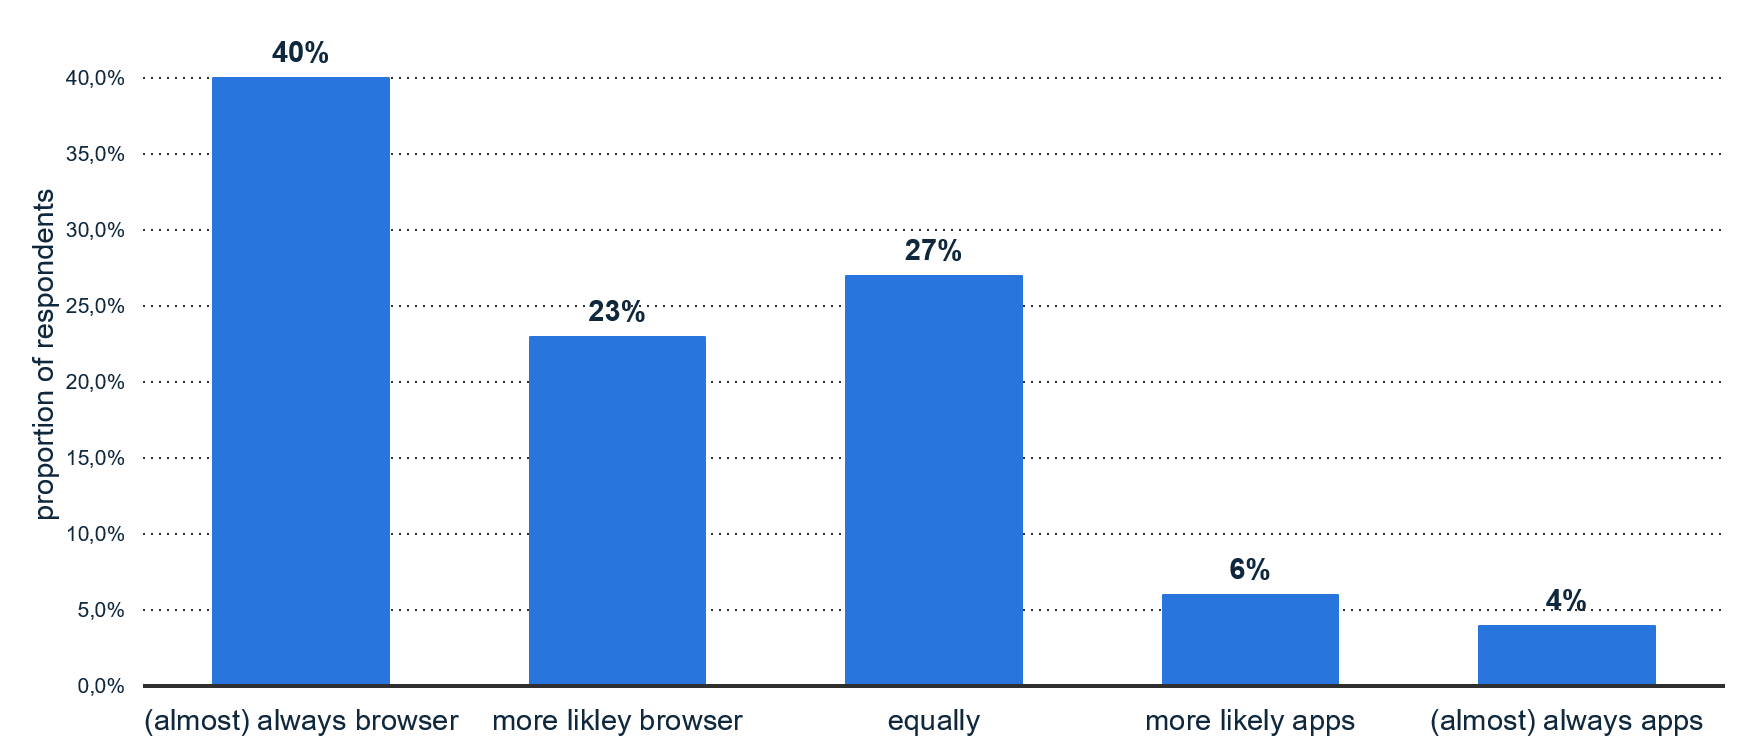
\includegraphics[width=\textwidth]{./Images/mia_browser_vs_apps_diagram.png}
	\end{center}
	\caption{Comparison graph: "Considering online shopping on mobile devices, are you more likely to use a browser applications or custom shop applications?"~\cite[The survey question as well as the captions of the graph are translated to english in a contextual manner.]{nutzungeinesbrowsersshopeigenerapp_06.08.2019}}
	\label{fig:comparison-mia-browser-vs-apps-diagram}
\end{figure}

\chapter{Appendixes}
\label{ch:appendixes}

\listoffigures % List of figures

\printacronyms % List of acronyms (defined in Acronyms.tex file)

\listoftables % List of tables

\bibliography{./Ressourcen/bibliography_example.bib} % Add your .bib file here

\end{document}